\begin{filecontents}{references.bib}
@article{riess1998,
  title={Observational evidence from supernovae for an accelerating universe and a cosmological constant},
  author={Riess, Adam G and Filippenko, Alexei V and Challis, Peter and Clocchiatti, Alejandro and Diercks, Alan and Garnavich, Peter M and Gilliland, Ron L and Hogan, Craig J and Jha, Saurabh and Kirshner, Robert P and others},
  journal={The astronomical journal},
  volume={116},
  number={3},
  pages={1009},
  year={1998},
  publisher={IOP Publishing}
}

@article{perlmutter1999,
  title={Measurements of $\Omega$ and $\Lambda$ from 42 high-redshift supernovae},
  author={Perlmutter, Saul and Aldering, Goldhaber and Goldhaber, Gerson and Knop, Richard A and Nugent, Peter and Castro, Patricia G and Deustua, Susana and Fabbro, Sebastien and Goobar, Ariel and Groom, Donald E and others},
  journal={The Astrophysical Journal},
  volume={517},
  number={2},
  pages={565},
  year={1999},
  publisher={IOP Publishing}
}

@article{perlmutter2003,
  title={Measuring cosmology with supernovae},
  author={Perlmutter, Saul and Schmidt, Brian P},
  journal={Supernovae and Gamma-Ray Bursters},
  pages={195--217},
  year={2003},
  publisher={Springer}
}

@book{weinberg2008,
  title={Cosmology},
  author={Weinberg, Steven},
  year={2008},
  publisher={OUP Oxford}
}

@article{straumann2012,
  title={The 2011 Nobel Prize in Physics},
  author={Straumann, Norbert and Z{\"u}rich, Uni},
  journal={SPG Mitteilungen},
  number={36},
  year={2012}
}

@article{betoule2014,
  title={Improved cosmological constraints from a joint analysis of the SDSS-II and SNLS supernova samples},
  author={Betoule, MEA and Kessler, R and Guy, J and Mosher, J and Hardin, D and Biswas, R and Astier, P and El-Hage, P and Konig, M and Kuhlmann, S and others},
  journal={Astronomy \& Astrophysics},
  volume={568},
  pages={A22},
  year={2014},
  publisher={EDP Sciences}
}

@article{siegel1982,
  title={Robust regression using repeated medians},
  author={Siegel, Andrew F},
  journal={Biometrika},
  volume={69},
  number={1},
  pages={242--244},
  year={1982},
  publisher={Oxford University Press}
}

@article{verde2019,
  title={Tensions between the early and late Universe},
  author={Verde, Licia and Treu, Tommaso and Riess, Adam G},
  journal={Nature Astronomy},
  volume={3},
  number={10},
  pages={891--895},
  year={2019},
  publisher={Nature Publishing Group UK London}
}

@article{abbott2024,
  title={The Dark Energy Survey: Cosmology Results With $\sim$1500 New High-redshift Type Ia Supernovae Using The Full 5-year Dataset},
  author={DES-Collaboration and Abbott, TMC and Acevedo, M and Aguena, M and Alarcon, A and Allam, S and Alves, O and Amon, A and Andrade-Oliveira, F and Annis, J and Armstrong, P and others},
  journal={arXiv preprint arXiv:2401.02929},
  year={2024}
}

@article{perivolaropoulos2022,
  title={Challenges for $\Lambda$CDM: An update},
  author={Perivolaropoulos, Leandros and Skara, Foteini},
  journal={New Astronomy Reviews},
  volume={95},
  pages={101659},
  year={2022},
  publisher={Elsevier}
}

@article{flaugher2015,
  title={The dark energy camera},
  author={Flaugher, Brenna and Diehl, HT and Honscheid, K and Abbott, TMC and Alvarez, O and Angstadt, R and Annis, JT and Antonik, M and Ballester, O and Beaufore, L and others},
  journal={The Astronomical Journal},
  volume={150},
  number={5},
  pages={150},
  year={2015},
  publisher={IOP Publishing}
}

@article{vincenzi2024,
  title={The Dark Energy Survey Supernova Program: Cosmological Analysis and Systematic Uncertainties},
  author={Vincenzi, M and Brout, D and Armstrong, P and Popovic, B and Taylor, G and Acevedo, M and Camilleri, R and Chen, R and Davis, TM and Lee, J and others},
  journal={The Astrophysical Journal},
  volume={975},
  number={1},
  pages={86},
  year={2024},
  publisher={IOP Publishing}
}

@article{shao2013,
  title={The energy loss of photons and cosmological redshift},
  author={Shao, Ming-Hui},
  journal={Physics Essays},
  volume={26},
  number={2},
  pages={183--190},
  year={2013},
  publisher={Physics Essays Publication}
}

@article{white2024,
  title={The Dark Energy Survey Supernova Program: Slow supernovae show cosmological time dilation out to $ z \sim 1$},
  author={White, Ryan MT and Davis, Tamara M and Lewis, Geraint F and Lidman, Christopher and Shah, Paul and Abbott, TMC and Aguena, M and Allam, S and Andrade-Oliveira, F and Asorey, J and others},
  journal={arXiv preprint arXiv:2406.05050},
  year={2024}
}

@article{blondin2008,
  title={Time dilation in type Ia supernova spectra at high redshift},
  author={Blondin, Stephanie and Davis, Tamara M and Krisciunas, Kevin and Schmidt, Brian P and Sollerman, J and Wood-Vasey, WM and Becker, AC and Challis, P and Clocchiatti, A and Damke, G and others},
  journal={The Astrophysical Journal},
  volume={682},
  number={2},
  pages={724},
  year={2008},
  publisher={IOP Publishing}
}

@article{zwicky1929,
  title={On the redshift of spectral lines through interstellar space},
  author={Zwicky, Fritz},
  journal={Proceedings of the National Academy of Sciences},
  volume={15},
  number={10},
  pages={773--779},
  year={1929},
  publisher={National Acad Sciences}
}

@article{tolman1930,
  title={On the estimation of distances in a curved universe with a non-static line element},
  author={Tolman, Richard C},
  journal={Proceedings of the National Academy of Sciences},
  volume={16},
  number={7},
  pages={511--520},
  year={1930},
  publisher={National Acad Sciences}
}

@article{desitter1934,
  title={On distance, magnitude, and related quantities in an expanding universe},
  author={de Sitter, Willem},
  journal={Bulletin of the Astronomical Institutes of the Netherlands, Vol. 7, p. 205},
  volume={7},
  pages={205},
  year={1934}
}

@article{hubble1935,
  title={Two methods of investigating the nature of the nebular redshift},
  author={Hubble, Edwin and Tolman, Richard C},
  journal={Astrophysical Journal, vol. 82, p. 302},
  volume={82},
  pages={302},
  year={1935}
}

@article{oke1968,
  title={Energy distributions, k corrections, and the Stebbins-Whitford effect for giant elliptical galaxies},
  author={Oke, John Beverley and Sandage, Allan},
  journal={Astrophysical Journal, vol. 154, p. 21},
  volume={154},
  pages={21},
  year={1968}
}

@article{kim1996,
  title={A generalized K correction for type Ia supernovae: comparing R-band photometry beyond z= 0.2 with B, V, and R-band nearby photometry},
  author={Kim, Alex and Goobar, Ariel and Perlmutter, Saul},
  journal={Publications of the Astronomical Society of the Pacific},
  volume={108},
  number={720},
  pages={190},
  year={1996},
  publisher={IOP Publishing}
}

@article{hsiao2007,
  title={K-corrections and spectral templates of Type Ia supernovae},
  author={Hsiao, Eric Y and Conley, A and Howell, DA and Sullivan, M and Pritchet, CJ and Carlberg, RG and Nugent, PE and Phillips, MM},
  journal={The Astrophysical Journal},
  volume={663},
  number={2},
  pages={1187},
  year={2007},
  publisher={IOP Publishing}
}

@article{kessler2009,
  title={SNANA: A public software package for supernova analysis},
  author={Kessler, Richard and Bernstein, Joseph P and Cinabro, David and Dilday, Benjamin and Frieman, Joshua A and Jha, Saurabh and Kuhlmann, Stephen and Miknaitis, Gajus and Sako, Masao and Taylor, Matt and others},
  journal={Publications of the Astronomical Society of the Pacific},
  volume={121},
  number={883},
  pages={1028},
  year={2009},
  publisher={IOP Publishing}
}

@article{burns2010,
  title={The Carnegie supernova project: light-curve fitting with SNooPy},
  author={Burns, Christopher R and Stritzinger, Maximilian and Phillips, MM and Kattner, ShiAnne and Persson, SE and Madore, Barry F and Freedman, Wendy L and Boldt, Luis and Campillay, Abdo and Contreras, Carlos and others},
  journal={The Astronomical Journal},
  volume={141},
  number={1},
  pages={19},
  year={2010},
  publisher={IOP Publishing}
}

@article{planck2015,
  title={Planck 2015 results-xiii. cosmological parameters},
  author={Planck-Collaboration and Ade, Peter AR and Aghanim, Nabila and Arnaud, M and Ashdown, Mark and Aumont, Jea and Baccigalupi, Carlo and Banday, AJ and Barreiro, RB and Bartlett, JG and Bartolo, Nicola and others},
  journal={Astronomy \& Astrophysics},
  volume={594},
  pages={A13},
  year={2016},
  publisher={EDP sciences}
}

@article{planck2020,
  title={Planck 2018 results-VI. Cosmological parameters},
  author={Planck-Collaboration and Aghanim, Nabila and Akrami, Yashar and Ashdown, Mark and Aumont, Jonathan and Baccigalupi, Carlo and Ballardini, Mario and Banday, Anthony J and Barreiro, RB and Bartolo, Nicola and Basak, S and others},
  journal={Astronomy \& Astrophysics},
  volume={641},
  pages={A6},
  year={2020},
  publisher={EDP sciences}
}

@article{camarena2020,
  title={Local determination of the Hubble constant and the deceleration parameter},
  author={Camarena, David and Marra, Valerio},
  journal={Physical Review Research},
  volume={2},
  number={1},
  pages={013028},
  year={2020},
  publisher={APS}
}

@book{peebles2020,
  title={Cosmology’s century: An inside history of our modern understanding of the universe},
  author={Peebles, Phillip James Edwin},
  year={2020},
  publisher={Princeton University Press}
}

@article{lesser2015,
  title={A summary of charge-coupled devices for astronomy},
  author={Lesser, Michael},
  journal={Publications of the Astronomical Society of the Pacific},
  volume={127},
  number={957},
  pages={1097--1104},
  year={2015},
  publisher={The Astronomical Society of the Pacific}
}
\end{filecontents}

\documentclass[aps,prl,reprint,amsmath,floatfix]{revtex4-2}

\usepackage{graphicx}
\usepackage{relsize}

\begin{document}

\title{Correcting K-correction: dark energy is based on a math error from 1930}

\author{Logan P. Evans}
 \email{loganpevans@gmail.com}
 \noaffiliation

\date{\today}

\begin{abstract}
We rederive the K-correction equation and discover that the version commonly
used to calculate magnitudes fails to account for time dilation. This error
traces back to 1930. We conclude that correcting apparent magnitudes for time
dilation resolves two of the preeminent mysteries in cosmology: first, dark
energy is not supported by observations of Type Ia supernovae and second, the
Hubble tension is due to the error in the K-correction equation.
\end{abstract}

\maketitle

\section{Introduction}

Cosmic expansion redshifts light, so when we compute the light travel distance
it is necessary to account for multiple redshift effects. We will show that
modern cosmology does not correct observations for time dilation.

Most cosmological models require an estimate of distance, so this error is far
reaching. However, we will focus on showing that correcting observations of
Type Ia supernovae (SNe Ia) for time dilation resolves the Hubble tension. The
Hubble tension, as described by \citet{verde2019}, is an observation that
independent techniques of estimating the expansion rate produce incompatible
values.

In order to use SNe Ia to estimate the expansion rate of the universe, we need
to identify both the redshift $z$ and the light travel distance $d_{LT}$. In
order to compute the light travel distance $d_{LT}$ in parsecs (pc), we use the
definition of the distance modulus \citep{weinberg2008}:

\begin{equation}
\label{eq:mu_def}
  d_{LT} = 10^{1 + (m - M)/5} \text{pc}.
\end{equation}

\noindent The quantity $m$ represents the apparent magnitude while $M$
represents the absolute magnitude of a SN Ia. It is common to use the
substitution $\mu = m - M$ and call $\mu$ the distance modulus.

Cosmology uses multiple distance measurements, but for measuring the expansion
rate of the universe, the only one we care about is the light travel distance
$d_{LT}$. A similar distance measurement, the luminosity distance $d_L$, is
often discussed in conjunction of flux measurements, but $d_L$ represents an
illusory distance. In fact, ${d_{L} = d_{LT} \times (1 + z)}$, which can be
thought of as the distance an object would need to be to produce the same
amount of measured energy flux if redshift did not exist. The light travel
distance $d_{LT}$ represents a physical quantity while $d_{L}$ does not.

Labeling $m$ as the ``apparent magnitude'' is a bit misleading for distant
observations because redshift will change several aspects of the observed
light. However, we can correct the value $m$ for redshift effects by using the
K-correction equation. This allows us to report an apparent magnitude that
represents the brightness of an object as if none of the light-altering effects
of redshift were present. According to \citet{riess1998}:

\begin{quote}
  An appropriate K-correction quantifies the \emph{difference} between the supernova
  light that falls into a standard passband (e.g., $B$) at ${z = 0}$ and that
  which falls into the filters we employ to observe a redshifted SN Ia.
\end{quote}

\noindent In other words, the goal of the K-correction equation is to remove
all redshift effects from the apparent magnitude $m$ so that the distance
modulus defined in Equation \ref{eq:mu_def} allows us to compute the light
travel distance $d_{LT}$.

\citet{tolman1930} published the first formal derivation of K-correction, but
he did not account for spectral bandwidth stretching, one of the dimming
effects of redshift. An alternative K-correction was correctly derived by
\citet{desitter1934}. However, in \citet{hubble1935}, the discrepancy between
the two equations was briefly discussed yet ultimately dismissed.
\citet{oke1968} derived a K-correction equation that they noted was equivalent
to earlier work, and while they accounted for spectral bandwidth stretching,
they did not account for time dilation. The paper by \citet{kim1996}, which is
the basis for modern implementations of K-correction, extended the work of
\citet{oke1968} to handle additional cross-filter comparisons and added a term
that addresses zero-point corrections.

The effect of using an incorrect redshift correction for SNe Ia is that we think
objects are farther away than they really are; this effect compounds for
greater distances. Up until \citet{riess1998}, we did not have distant enough
observations for this error to matter much for cosmological models, but by the
late 1990s, it became clear that our measurements for distance and redshift
were not linear. This realization led to a model that utilized a cosmological
constant $\Lambda$ and dark energy in order to explain the non-linear
distance-redshift graph. We will show that correcting the flaws of K-correction
leads to a linear graph that does not need to rely on a cosmological constant.

\citet{planck2015} used an alternative technique to compute the Hubble constant
$H_0$ that is based on measurements of the cosmic microwave background (CMB).
CMB-based computations of $H_0$ have made it evident that something is missing
with our understanding of cosmology because this technique produces a
significantly different value than when the constant is derived using SNe Ia.
Fixing the errors with K-correction produces a measurement of the Hubble
constant that is compatible with models based on the CMB.

\section{A brief history of K-correction}

Observational data from SNe Ia are essential for the calibration of models that
use redshift to estimate distance. The approximately linear relationship
between redshift and light travel distance, often called the
Hubble-Lema\^{i}tre law, describes how quickly the universe is expanding.
However, \citet{riess1998} and \citet{perlmutter1999} presented evidence that
there is not a linear relationship between redshift and distance, but instead,
distant objects are farther away than their redshift would predict (see Figure
\ref{fig:distance_vs_redshift}). This phenomenon implies that the
acceleration of the universe is faster today than it was for old observations.
The cause of this phenomenon was unknown and was referred to as dark energy.

\begin{figure}
  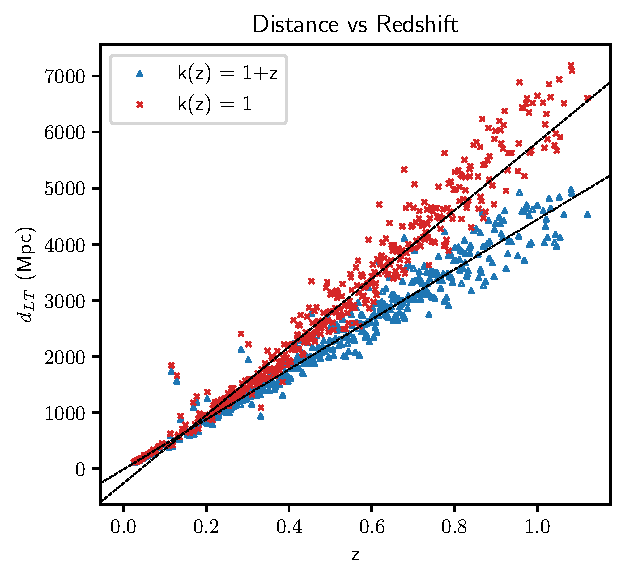
\includegraphics[width=\columnwidth]{distance_vs_redshift.pdf}
  \caption {The relationship between light travel distance $d_{LT}$ and
  redshift $z$ for two treatments of the magnitude data. The red ${k(z) = 1}$
  treatment, which represents the uncorrected values, is clearly non-linear
  while the blue ${k(z) = 1 + z}$ treatment, which fixes the K-correction
  redshift error, appears to be linear.  The displayed points are roughly a
  third of the values in the full SNe Ia dataset published in
  \citet{abbott2024}, selected with uniform redshift spacing to aid visibility.
  }
  \label{fig:distance_vs_redshift}
\end{figure}

SNe Ia are used to explore the relationship between distance and redshift because
these events have a roughly constant absolute magnitude which allows us to use
the apparent magnitude to estimate distance.

However, redshifting dims the brightness of an observation in three ways:

\begin{itemize}
  \item The energy of a wave is inversely proportional to its wavelength; thus a
  redshift of $z$ means the amount of energy per photon is reduced by a factor
  of ${1 / (1+z)}$.

  \item The bandwidth stretches. If the rest frame observes photons in the
  bandwidth from 400nm and 401nm, then a redshift of ${z = 1}$ stretches the
  wavelengths to the bandwidth from 800nm to 802nm. The number of photons per
  bandwidth is reduced by a factor of ${1 / (1+z)}$.

  \item Cosmological time dilation reduces the rate at which photons arrive.
  The number of photons that arive per second is reduced by a factor of ${1 / (1+z)}$.
\end{itemize}

To complicate matters, we use the $B$ band magnitude to calculate light travel
distance. We want to know how bright a supernova appears for wavelengths around
445nm as if no redshift had occurred. However, we typically need to observe the
supernova with a filter that is sensitive to longer wavelengths, such as the
$i$ band filter which is sensitive to wavelengths from 700nm-850nm
\citep{flaugher2015}. The K-correction formula allows us to take a magnitude
measured in an observation filter $y$ and compute the magnitude in the target
filter $x$. Even if the observation filter is the same as the target filter,
the K-correction equation is necessary to remove redshift effects.

The first mathematical treatment of K-correction was performed by
\citet{tolman1930}. However, when Tolman made his derivation, he did not
consider the effects of a spectrum that is stretched due to redshift.

A few years later, \citet{desitter1934} discussed all three issues that reduce
the observed brightness of a distant observation. The correction for each of
these issues is identical: take a flux measurement and multiply it by the
factor $1 + z$.

A year later, \citet{hubble1935} published a similar set of calculations where
they stated:

\begin{quote}
It should be specially noted that this expression differs from the correction
to $m$ proposed by de Sitter, which contains the term $(1 + z)^3$ instead of
$(1 + z)^2$. Expression (28), however, would seem to give the proper correction
to use in connection with our equation (21), since it has been derived in such
a way as to make appropriate allowance, first, for the double effect of nebular
recession in reducing both the individual energy and the rate of arrival of
photons, and then for the further circumstance that a change in spectral
distribution of the energy that does arrive will lead to changes in its
photographic effectiveness.
\end{quote}

\noindent However, even though they considered all three dimming effects of
redshift, they started their derivation by copying the incorrect equation from
1930. The incorrect correction term has been used ever since.

In a paper published by \citet{oke1968}, the two factors of ${1 + z}$ were
attributed to the change in energy and to the spectral bandwidth elongation,
which leaves time dilation as the factor that was omitted.

The modern treatment of K-correction is based on the work of \citet{kim1996}.
This work extended the work of \citet{oke1968} to apply to filters beyond the
blue $B$ and visible $V$ bands. It also introduced a term that deals with the
zero-point correction for the actual filters. Historically, bolometric devices
would measure the energy flux, but modern charge-coupled device (CCD) cameras
effectively measure the photon flux, so \citet{kim1996} derived a form of the
K-correction equation that uses photon flux. This is the form of the
K-correction equation that is used by modern astrophysics, but we will show
that this equation still contains the time dilation error that produces the
dark energy phenomenon.

\section{Derivation of K-correction}

The K-correction $K_{xy}$ uses a spectral energy density template $F$ that
specifies the expected spectrum for a SN Ia observation. It also uses the
observed redshift $z$ and the observed photon flux magnitude $m_y$ measured in
filter $y$.

With modern CCD cameras, a telescope observation consists of a single value
$\mathcal{F}_y$ erg/s, which represents the energy collected per second in
filter $y$. Photogenerated electrons are collected in potential wells, which
means that the energy measured in this filter is proportional to the number of
photons \citep{lesser2015}. However, we need to calculate the expected number
of photons collected by using a spectral energy density function $F$.

\begin{figure}
  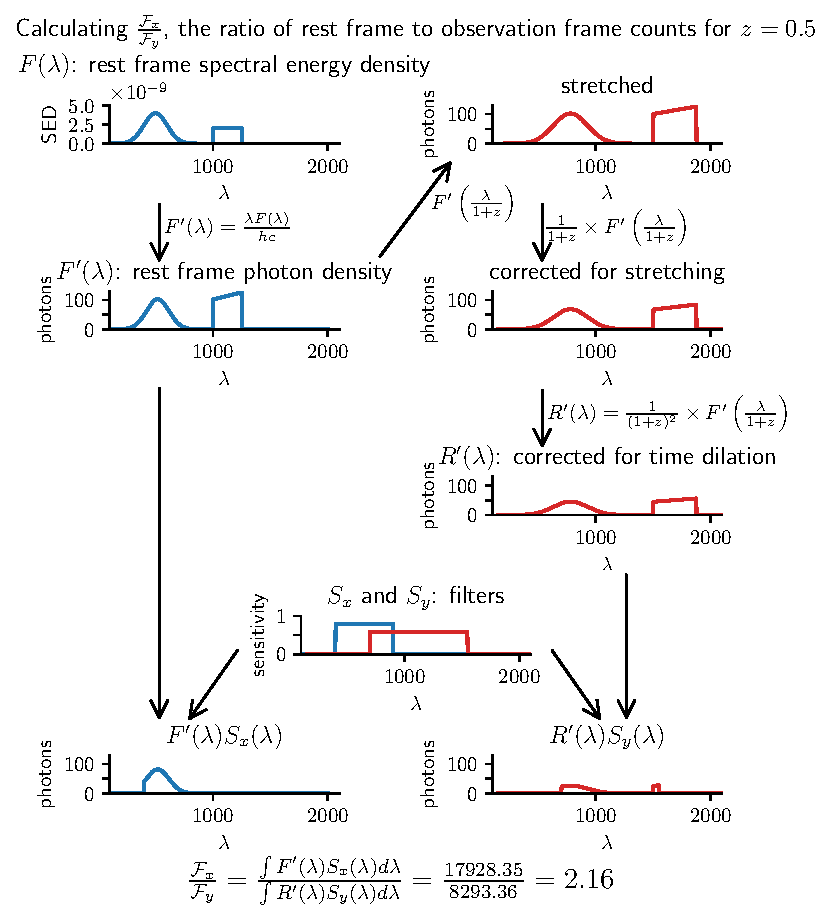
\includegraphics[width=\columnwidth]{k_equation_flow.pdf}
  \caption{The value $\mathcal{F}_x / \mathcal{F}_y$ is equal to the number of
  photons we want to report in the target filter divided by the number of
  photons we measure in the observation filter. Deriving this value starts with
  $F(\lambda)$, the spectral energy density, which we then convert to
  $F'(\lambda)$, the photon density for the rest frame. Starting at the top
  right corner of the figure we show three steps used to compute $R'(\lambda)$,
  the photon density in the observation frame. We first stretch the photon
  density, but this step inflates counts. In the second step, we correct for
  the inflated counts by multiplying by $1/(1+z)$; at this point, the total
  count equals the total count of $F'(\lambda)$. Finally, in the third step we
  finish calculating the observation frame photon density $R'(\lambda)$ by
  accounting for time dilation, which also reduces photon counts by a factor of
  $1/(1+z)$. We can compute the expected ratio of photons by totalling the area
  under the curves in the bottom two panels. Dark energy occurs when we omit
  the step that corrects for time dilation.
  }
  \label{fig:k-example}
\end{figure}

To convert the spectral energy density $F$ to the photon density $F'$, we need
to use the Plank relation $E = hc / \lambda$ where $E$ is the energy, $h$
is Planck's constant, and $c$ is the speed of light. This gives us

\begin{equation}
\begin{aligned}
\label{eq:eflux2pflux}
   F(\lambda) &= F'(\lambda) \times \frac{hc}{\lambda} \\
  F'(\lambda) &= \frac{\lambda F(\lambda)}{hc}.
\end{aligned}
\end{equation}

It is important to note that for the blueshifted wavelength $\lambda / (1+z)$,
this equation produces

\begin{equation}
 F'\left(\frac{\lambda}{1+z}\right) = \frac{\lambda}{(1+z)hc} F\left(\frac{\lambda}{1+z}\right).
\end{equation}

\noindent However, this equation is misleading and error prone. We will want to
use it to help calculate the flux in an observation filter at the redshifted
wavelength $\lambda \times (1 + z)$. In other words, we want to produce the
photon density function $R'$ that is the redshifted version of $F'$.
Redshifting the photon density does two things:

\begin{itemize}
  \item All wavelengths are increased by a factor of $1 + z$. When we integrate
  $R'$ from wavelength $\lambda_a$ to wavelength $\lambda_b$, the values
  correspond to the wavelengths $\lambda_a / (1+z)$ to $\lambda_b / (1+z)$ in
  $F'$. We will integrate over a width of $\lambda_b - \lambda_a$, but
  $F'(\lambda / (1+z))$ will refer to values in a width of
  $(\lambda_b - \lambda_a) / (1+z)$.

  In order to account for the spectral bandwidth stretching effect, we
  multiply $F'$ by $1/(1+z)$.

  \item The stretching of space increases the distance between photons while
  they are traveling. To an observer, this phenomenon appears like time
  dilation, although cosmological time dilation is due to a different mechanism
  than relativistic time dilation. This effect reduces the photon arrival rate
  by a factor of $1/(1+z)$.

  In order to account for cosmological time dilation, we multiply $F'$ by a
  second factor of $1/(1+z)$.
\end{itemize}

Combining these two phenomena, we can calculate the redshifted spectral energy
density $R$ using

\begin{equation}
\begin{aligned}
\label{eq:redshifted_density}
  R'(\lambda) &= F'\left(\frac{\lambda}{1+z}\right) \times \frac{1}{(1 + z)^2} \\
  R(\lambda) &= \frac{\lambda}{(1+z)hc} \times F\left(\frac{\lambda}{1+z}\right) \times \frac{1}{(1 + z)^2} .
\end{aligned}
\end{equation}

\noindent We deliberately do not combine all of the factors of $1+z$ together because
this form is more natural to implement in code.

In order to calculate the flux $\mathcal{F}_x$ measured in filter $x$, we need
to compute the photon density $F'(\lambda)$ and multiply it by the sensitivity
$S_x(\lambda)$, which represents the proportion of photons with wavelength
$\lambda$ that filter $x$ will measure. We then sum over all wavelengths, which
is expressed with the equation

\begin{equation}
\begin{aligned}
\label{eq:flux_definition}
  \mathcal{F}_x &= \int F'(\lambda) S_x(\lambda) d\lambda \\
                &= \int \lambda F(\lambda) S_x(\lambda) d\lambda.
\end{aligned}
\end{equation}

We will also use the flux $\mathcal{F}$ to magnitude $m$ formula:

\begin{equation}
\begin{aligned}
\label{eq:flux2mag}
                             m_x &= -2.5 \text{log}(\mathcal{F}_x) + P_x \\
  -2.5 \text{log}(\mathcal{F}_x) &= m_x - P_x .
\end{aligned}
\end{equation}

\noindent $P_x$ represents the zero-point for the filter $x$ on some particular
telescope. In order to use consistent magnitude values across telescopes that
have different light gathering abilities, we take the measured magnitude and
multiply it by the ratio of the standard flux rate to the flux rate for this
particular telescope and filter. For convenience, we use $P_x = -2.5
\text{log}(P'_x)$ so that we can work with flux instead of with magnitude.

Now that we have the identities in Equations \ref{eq:flux_definition} and
\ref{eq:flux2mag}, we will change directions and look at the definition of
K-correction $K_{xy}$. This value allows us to make an observation in filter
$y$ and report what the magnitude would have been in filter $x$ if no redshift
occurred:

\begin{equation}
\begin{aligned}
\label{eq:definition}
  m_y &= M_x + \mu + K_{xy} \\
      &= M_x + m_x - M_x + K_{xy} \\
      &= m_x + K_{xy} \\
  m_x &= m_y - K_{xy} .
\end{aligned}
\end{equation}

\noindent The second line of Equation \ref{eq:definition} expands the distance modulus
$\mu$ using $\mu = m - M$ where $m$ is the observed magnitude and $M$ is the
absolute magnitude.

Since the K-correction is a magnitude value and we wish to work on flux values,
it is convenient to define the following substitution:

\begin{equation}
\label{eq:k_substitution}
  K_{xy} = 2.5\text{log}(K'_{xy}) .
\end{equation}

\noindent Note that this substitution omits the minus ($-$) sign that we used on a
similar substitution for $P_x$.

Starting with Equation \ref{eq:flux2mag} and then
recombining the flux term $\mathcal{F}_y$ with $m_y$ from Equation
\ref{eq:definition}, we have

\begin{equation}
\begin{aligned}
\label{eq:as_flux}
  -2.5 \text{log}(\mathcal{F}_x)
      &= m_x - P_x \\
      &= m_y - K_{xy} - P_x \\
      &= -2.5 \text{log}(\mathcal{F}_y) + P_y - K_{xy} - P_x \\
      &= -2.5 \text{log}(\mathcal{F}_y) - 2.5 \text{log}(P'_y) \\
         &\qquad - 2.5 \text{log}(K'_{xy}) + 2.5 \text{log}(P'_x) \\
      &= -2.5 \left(\text{log}(\mathcal{F}_y) + \text{log}(K'_{xy}) \right. \\
         &\qquad\qquad + \left. \text{log}(P'_y) - \text{log}(P'_x)
        \right) \\
      &= -2.5 \text{log}\left(
        \mathcal{F}_y
        \times K'_{xy}
        \times \frac{P'_y}{P'_x}\right) \\
  \mathcal{F}_x &= \mathcal{F}_y \times K'_{xy} \times \frac{P'_y}{P'_x}.
\end{aligned}
\end{equation}

\noindent We can isolate $K'_{xy}$ and then use Equation \ref{eq:flux_definition} to expand

\begin{equation}
\begin{aligned}
  \mathcal{F}_x &= \mathcal{F}_y \times K'_{xy} \times \frac{P'_y}{P'_x} \\
        K'_{xy} &= \frac{P'_x}{P'_y} \times \frac{\mathcal{F}_x}{\mathcal{F}_y} .
\end{aligned}
\end{equation}

\noindent We now use Equations \ref{eq:redshifted_density} and \ref{eq:flux_definition}
to calculate the fluxes $\mathcal{F}_x$ and $\mathcal{F}_y$ in terms of the
spectral energy density function $F$. Note that $\mathcal{F}_x$ uses the rest
frame spectral energy density $F$, while $\mathcal{F}_y$ uses the redshifted
spectral energy density $R(\lambda)$:

\begin{equation}
\begin{aligned}
  K'_{xy} &= \frac{P'_x}{P'_y} \times \frac{\mathcal{F}_x}{\mathcal{F}_y} \\
          &= \frac{P'_x}{P'_y} \times
              \frac{\int F'(\lambda) S_x(\lambda) d\lambda}
                   {\int R'(\lambda) S_y(\lambda) d\lambda} \\
          &= \frac{P'_x}{P'_y} \times
              \frac{\int F'(\lambda) S_x(\lambda) d\lambda}
                   {\int F'\left(\frac{\lambda}{1+z}\right) \times \left(\frac{1}{1 + z}\right)^2 S_y(\lambda) d\lambda} \\
          &= \frac{P'_x}{P'_y} \times (1+z)^2 \times
              \frac{\int \left(\frac{\lambda}{hc}\right) F(\lambda) S_x(\lambda) d\lambda}
                   {\int \frac{\lambda}{(1+z)hc} F\left(\frac{\lambda}{1+z}\right) S_y(\lambda) d\lambda} \\
          &= \frac{P'_x}{P'_y} \times (1 + z)^2 \times
              \frac{\int \lambda F(\lambda) S_x(\lambda) d\lambda}
                   {\int \left(\frac{\lambda}{1+z}\right) F\left(\frac{\lambda}{1+z}\right) S_y(\lambda) d\lambda} .
\end{aligned}
\end{equation}

Finally, we use Equation \ref{eq:k_substitution} to convert $K'_{xy}$ back into
the magnitude $K_{xy}$:

\begin{equation}
\begin{aligned}
\label{eq:K2k}
  K_{xy} &= 2.5\text{log}(K'_{xy}) \\
         &= 2.5\text{log}
  \begin{aligned}[t]
          &\left( \vphantom{\frac{\int}{\left(\frac{\int}{1}\right)}} \right.
              \frac{P'_x}{P'_y} \times (1 + z)^2 \\
          &\left.\quad \times
              \frac{\int \lambda F(\lambda) S_x(\lambda) d\lambda}
                   {\int \left(\frac{\lambda}{1+z}\right) F\left(\frac{\lambda}{1+z}\right) S_y(\lambda) d\lambda}\right)
  \end{aligned} \\
         &= 2.5
  \begin{aligned}[t]
         &\left( \vphantom{\frac{\int}{\left(\frac{\int}{1}\right)}}
            \text{log} \left( \frac{P'_x}{P'_y} \right)
            + \text{log}\left( {(1 + z)^2}\right) \right. \\
         &\left.\quad + \text{log}\left( \frac{\int \lambda F(\lambda) S_x(\lambda) d\lambda}
                                    {\int \left(\frac{\lambda}{1+z}\right) F\left(\frac{\lambda}{1+z}\right) S_y(\lambda) d\lambda}
            \right) \right)
  \end{aligned} \\
         &= 2.5 \text{log} \left( \frac{P'_x}{P'_y} \right)
            + 5 \text{log} (1 + z) \\
            &\quad + 2.5 \text{log} \left(
              \frac{\int \lambda F(\lambda) S_x(\lambda) d\lambda}
                   {\int \frac{\lambda}{1+z} F\left(\frac{\lambda}{1+z}\right) S_y(\lambda) d\lambda} \right) \\
         &= 5 \text{log} (1 + z)
            + 2.5 \text{log} \left(
              \frac{\int \lambda F(\lambda) S_x(\lambda) d\lambda}
                   {\int \frac{\lambda}{1+z} F\left(\frac{\lambda}{1+z}\right) S_y(\lambda) d\lambda} \right) \\
            &\quad - P_x + P_y .
\end{aligned}
\end{equation}

\section{Consequences}

The modern version of the K-correction equation was presented by \citet{kim1996}:

\begin{equation}
\begin{aligned}
\label{eq:kim}
  K_{xy} &=
    -2.5\text{log} \left(
      \frac{\int \lambda \mathcal{Z}(\lambda)S_x(\lambda)d\lambda}
           {\int \lambda \mathcal{Z}(\lambda)S_y(\lambda)d\lambda}\right) \\
    &\quad + 2.5\text{log}(1+z) \\
    &\quad + 2.5\text{log}\left(
      \frac{\int \lambda F(\lambda)S_x(\lambda)d\lambda}
           {\int \lambda F\left(\frac{\lambda}{1+z}\right)S_y(\lambda)d\lambda}\right) \quad \text{(incorrect)}.
\end{aligned}
\end{equation}

In order to fully compare Equation \ref{eq:K2k} against Equation \ref{eq:kim},
we need to convert the zero-point value $P_x$ into an expression that describes
the accumulation of flux $\mathcal{F}_x$. We start with
Equation \ref{eq:flux2mag}, set ${m_x = 0}$, and solve for the zero-point value
$P_x$:

\begin{equation}
\begin{aligned}
  m_x &= -2.5 \text{log}(\mathcal{F}_x) + P_x \\
    0 &= -2.5 \text{log}(\mathcal{F}_x) + P_x \\
  P_x &= 2.5 \text{log}(\mathcal{F}_x).
\end{aligned}
\end{equation}

\noindent Next, we convert the measured flux $\mathcal{F}_x$ to energy flux
$F_x$ using Equation \ref{eq:flux_definition} before renaming
$F(\lambda) = \mathcal{Z}(\lambda)$ to indicate that we are measuring the
idealized zero-point flux.

\begin{equation}
\begin{aligned}
  P_x &= 2.5 \text{log}(\mathcal{F}_x(\lambda)) \\
      &= 2.5 \text{log}\left( \int \lambda F(\lambda) S_x(\lambda) d\lambda \right) \\
      &= 2.5 \text{log}\left( \int \lambda \mathcal{Z}(\lambda) S_x(\lambda) d\lambda \right).
\end{aligned}
\end{equation}


\noindent Combining this with Equation \ref{eq:K2k}, we have

\begin{equation}
\begin{aligned}
  K_{xy} &= 5 \text{log} (1 + z) \\
          &\quad + 2.5 \text{log} \left(
              \frac{\int \lambda F(\lambda) S_x(\lambda) d\lambda}
                   {\int \frac{\lambda}{1+z} F\left(\frac{\lambda}{1+z}\right) S_y(\lambda) d\lambda} \right) \\
          &\quad - P_x + P_y \\
         &= 5 \text{log} (1 + z) \\
          &\quad + 2.5 \text{log} \left(
              \frac{\int \lambda F(\lambda) S_x(\lambda) d\lambda}
                   {\int \frac{\lambda}{1+z} F\left(\frac{\lambda}{1+z}\right) S_y(\lambda) d\lambda} \right) \\
          &\quad - 2.5 \text{log} \left( \int \frac{\lambda}{hc} \mathcal{Z}(\lambda) S_x(\lambda) d\lambda \right) \\
          &\quad + 2.5 \text{log} \left( \int \frac{\lambda}{hc} \mathcal{Z}(\lambda) S_y(\lambda) d\lambda \right) \\
         &= -2.5 \text{log} \left(
              \frac{\int \lambda \mathcal{Z}(\lambda) S_x(\lambda) d\lambda}
                   {\int \lambda \mathcal{Z}(\lambda) S_y(\lambda) d\lambda}
             \right) \\
          &\quad + 5 \text{log} (1 + z) \\
          &\quad + 2.5 \text{log} \left(
              \frac{\int \lambda F(\lambda) S_x(\lambda) d\lambda}
                   {\int \frac{\lambda}{1+z} F\left(\frac{\lambda}{1+z}\right) S_y(\lambda) d\lambda} \right) .
\end{aligned}
\end{equation}

Two differences with Equation \ref{eq:kim} stand out:

\begin{itemize}
  \item The second term is multiplied by $2.5$ in \citet{kim1996}, but is
  multiplied by $5$ here. This is the manifestation of the error in
  \citet{tolman1930} and leads to the conclusion that the expansion of the
  universe is accelerating.

  \item In our derivation, the third term has an extra $1 + z$ expression.
  Based on an inspection of the SN(oo)py software package presented by
  \citet{burns2010} and the SNANA software package presented by
  \citet{kessler2009}, this error is ignored and software package authors
  implement it as intended, not precisely as written.
\end{itemize}

\section{Conclusions}

\begin{figure}
  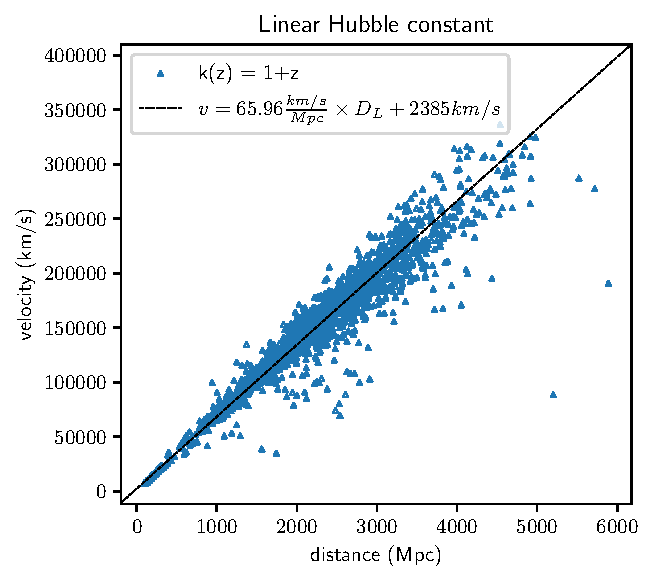
\includegraphics[width=\columnwidth]{velocity_vs_distance.pdf}
  \caption{The relationship between expansion velocity and light travel
  distance. The slope of this graph demonstrates the Hubble constant. The data
  for these SN Ia observations comes from the Dark Energy Survey
  \citep{vincenzi2024}, but the magnitudes are corrected to account for time
  dilation by adding ${-2.5 \text{log}(1 + z)}$.
  }
\label{fig:expansion}
\end{figure}

As shown in Figure \ref{fig:distance_vs_redshift}, when reported magnitudes
are corrected by adding the magnitude $-2.5\text{log}(1+z)$, there is a linear
relationship between redshift and light travel distance. This is in accordance
with the Hubble-Lema\^{i}tre law. As opposed to the uncorrected values, there
is no visual acceleration. Since the corrected values are approximately linear,
we can use them to estimate the Hubble constant $H_0$ which is demonstrated in
Figure \ref{fig:expansion}.

The value estimated here, $H_0 = 65.94 \pm 1.3$, is consistent with
estimates of $H_0$ that are based on the CMB. \citet{planck2020} published the
CMB value of $H_0 = 67.27 \pm 0.6$, and the one sigma error bars overlap.

Since the K-correction error has corrupted all astronomical measurements that
depend on both magnitude and redshift, a lot of data needs to be reanalysed.
Cosmological parameters, such as those used by the
Friedmann-Lema\^{i}tre-Robertson-Walker (FLRW) metric or the $\Lambda$-CDM
model, can only be recalculated once the data is cleaned.

The reasons that the K-correction errors went undiscovered for so long should
also be explored. Many hints existed that something was wrong, yet the
problems persisted.

\bibliography{references}

\end{document}

